% Chapter 2

\chapter{\uppercase{Design of the project }} % Main chapter title
\label{ch:survey} % For referencing

Project design is an early phase of the project where a projects key
features,structure,criteria for success and major deliverables are all planned out.The
point is to develop one or more designs which can be used to acheive the desired
project goals.
We have delivered the three main design models which depicts the
overall architectural structure and flow of our project in an interactive way.

System architecture - Application architecture is the high level structure
of an application system. Its the process of defining a structured solution that
meets all of the technical and operational requirements.

State diagram - It describes the behaviour of a single object in response
to series of events in the system.It depicts the dynamic flow from state to state
of particular object within system.

Sequence diagram - A sequence diagram is an interaction diagram
that shows how objects operate with one another and in what order.It shows
object interations arranged in time sequence.


\begin{center}
  %
\includegraphics[width=26mm,height=25mm]{auemblem.pdf}   \\
  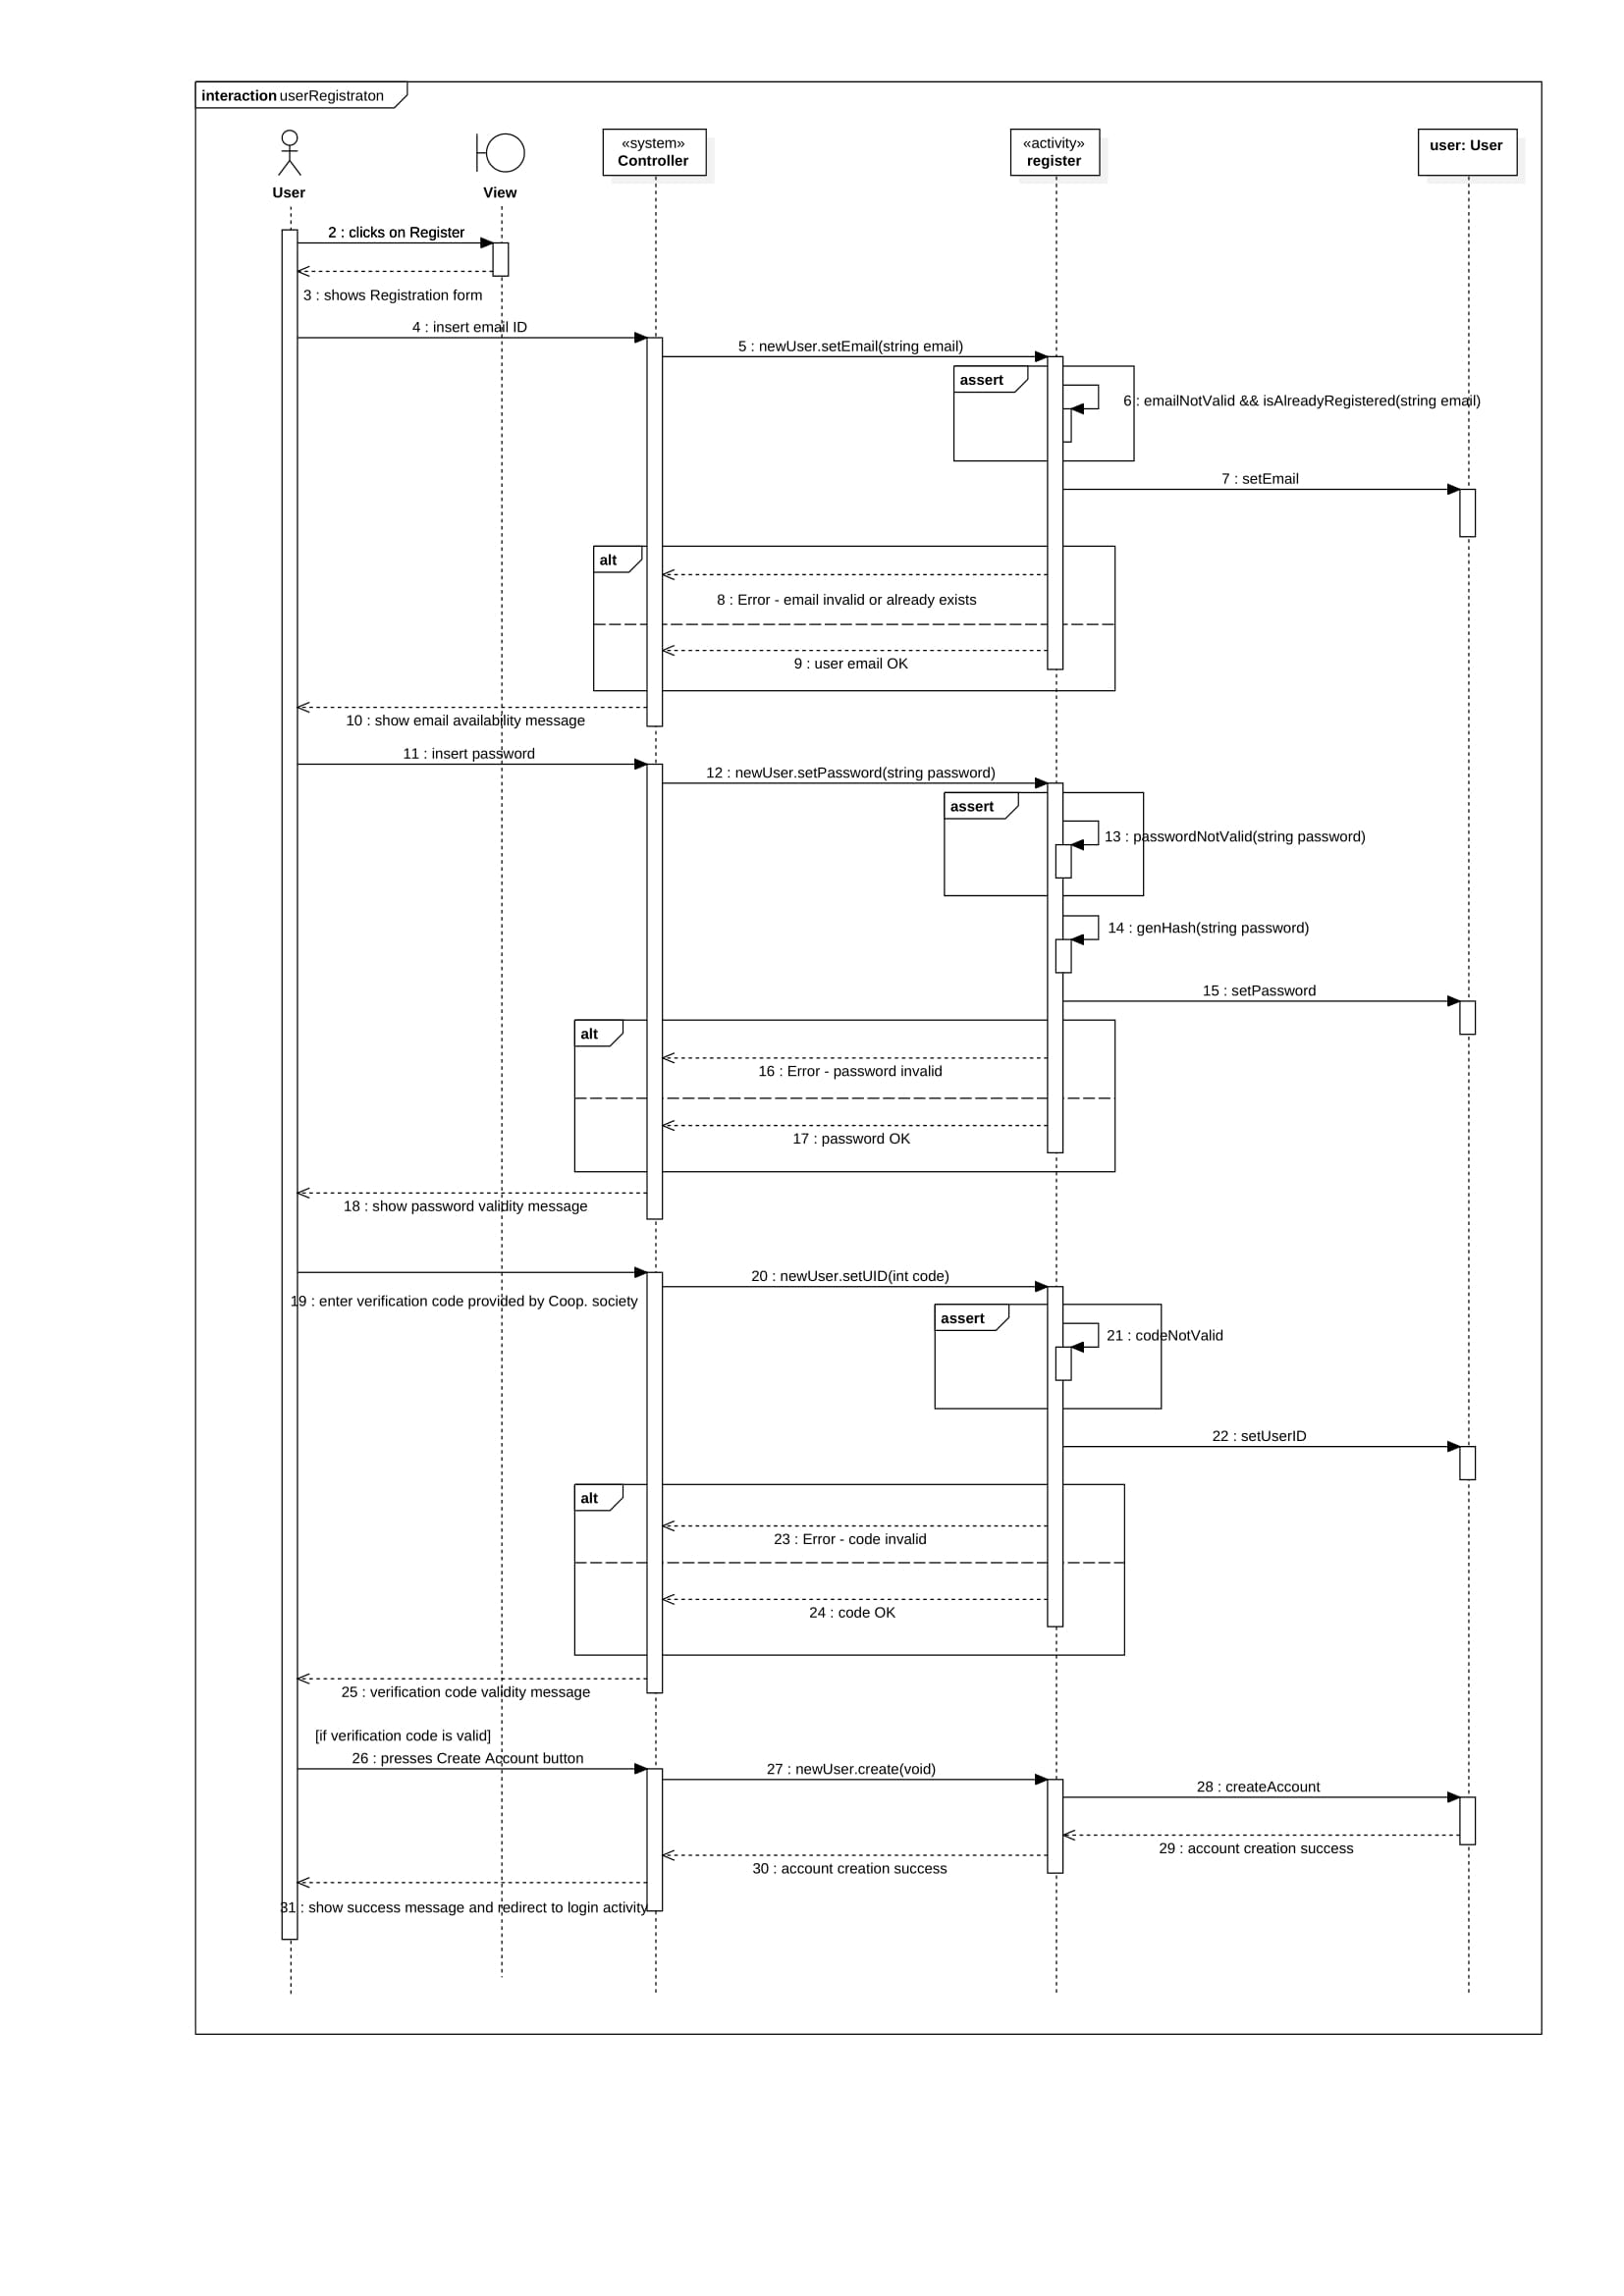
\includegraphics[scale=0.275]{user-registration-1.jpg} \\
\end{center}